\documentclass[conference]{IEEEtran}
\IEEEoverridecommandlockouts

\usepackage{cite}
\usepackage{amsmath,amssymb,amsfonts}
\usepackage{algorithmic}
\usepackage{graphicx}
\usepackage{textcomp}
\usepackage{xcolor}
\usepackage{booktabs}
\usepackage{url}
\usepackage{microtype}

\def\BibTeX{{\rm B\kern-.05em{\sc i\kern-.025em b}\kern-.08em
    T\kern-.1667em\lower.7ex\hbox{E}\kern-.125emX}}

\begin{document}

\title{Architecting Mixed-Evidence Automated Programming Assessment: Deterministic Guardrails, Algorithmic Complexity Reasoning, and Staged Pedagogical Guidance}

\author{\IEEEauthorblockN{A Manigreeva\IEEEauthorrefmark{1}, D Nayaneesh\IEEEauthorrefmark{1}, Kantam Pavan Sai Reddy\IEEEauthorrefmark{1}, Kura Vignesh Reddy\IEEEauthorrefmark{1}, Vitta Karthikeya\IEEEauthorrefmark{1}}
\IEEEauthorblockA{\IEEEauthorrefmark{1}Department of Computer Science and Engineering\\
Email: \{manigreeva, nayaneesh, pavansai, vigneshreddy, karthikeya\}@codeassessment.internal}
}

\maketitle

\begin{abstract}
Automated programming assessment systems face a fundamental dilemma: traditional test-suite autograders provide objective pass/fail verdicts but offer no pedagogical feedback or algorithmic efficiency analysis, while recent holistic Large Language Model (LLM) graders produce fluent explanations but suffer from stochastic score drift, ungrounded grading hallucinations, and answer disclosure that induces novice cognitive offloading. 

We present \textbf{CodeAssessment}, a mixed-evidence assessment architecture that rigorously decouples deterministic grading authority from generative pedagogical guidance. CodeAssessment executes student code inside containerized sandboxes (1.0~vCPU, 256\,MB RAM, 5.0\,s CPU limit) and computes functional correctness strictly from observable test verdicts. To evaluate algorithmic efficiency without benchmark contamination, we formulate a 10-level asymptotic rank ladder ($O(1)$ to $O(n!)$) with a scaled worse-penalty function driven by Tree-sitter Abstract Syntax Tree (AST) analysis and execution profiling. Composite grades are computed via a dynamically renormalized rubric with an enforced 79.0\% non-accepted cap, ensuring incorrect code cannot achieve high grades through style or efficiency alone. Crucially, generative LLM agents are restricted to non-grading roles: evidence-grounded diagnosis, curricular roadmap navigation, and staged pedagogical hints, backed by a deterministic structural fallback when LLM providers fail. 

We evaluate CodeAssessment against 194,550 records across 1,890 algorithmic problems, verifying 100\% test suite compliance across 265 automated test cases. Infrastructure colocation in the Mumbai region reduces query round-trip latency by 92.2\% (from 553.9\,ms to 43.18\,ms) and test execution time by 83.5\%. We report verified architectural findings alongside material limitations, including API benchmark leakage and execution fallback risks, establishing a reproducible blueprint for trustworthy, evidence-first autograding.
\end{abstract}

\begin{IEEEkeywords}
Automated code assessment, programming education, multi-agent systems, large language models, static analysis, explainability, reproducibility.
\end{IEEEkeywords}

\section{Introduction}
Providing timely, actionable feedback is a cornerstone of computer science education. For decades, automated assessment systems (AAS) have relied on input-output test suites to grade student assignments~\cite{keuning2018systematic, edwards2008webcat}. While test runners establish functional correctness on specific inputs, they operate as pedagogical black boxes: a zero score on a hidden test does not indicate whether the student suffered an off-by-one boundary flaw, an asymptotic time-limit timeout ($O(n^2)$ vs. $O(n \log n)$), or an unhandled recursion base case.

The rapid emergence of Large Language Models (LLMs) appeared to offer a solution. Recent efforts deploy LLMs as virtual tutors and holistic autograders~\cite{macneil2023codeexplanation, sahu2026autograder}. However, empirical investigations in computing education have exposed severe vulnerabilities in pure LLM grading. LLM evaluators exhibit non-deterministic grade drift on identical submissions, assign arbitrary numeric marks detached from rubrics, and are susceptible to prompt injection via student source comments~\cite{prather2023weird, becker2023programming}. Furthermore, when LLMs output complete revised code, students frequently copy solutions without conceptual engagement, inducing cognitive offloading~\cite{denny2024promptproblems}.

Recent software engineering frameworks assemble multi-agent LLM systems to coordinate complex tasks~\cite{wu2023autogen, hong2024metagpt}. Yet, in autograding, multi-agent decomposition often creates an \textit{orchestration mirage}: an unverified score generated by an LLM node (such as an imputed originality score or an unverified score projection) acquires the false illusion of scientific rigor simply because it was emitted by a named multi-agent graph.

\begin{figure*}[!t]
\centering
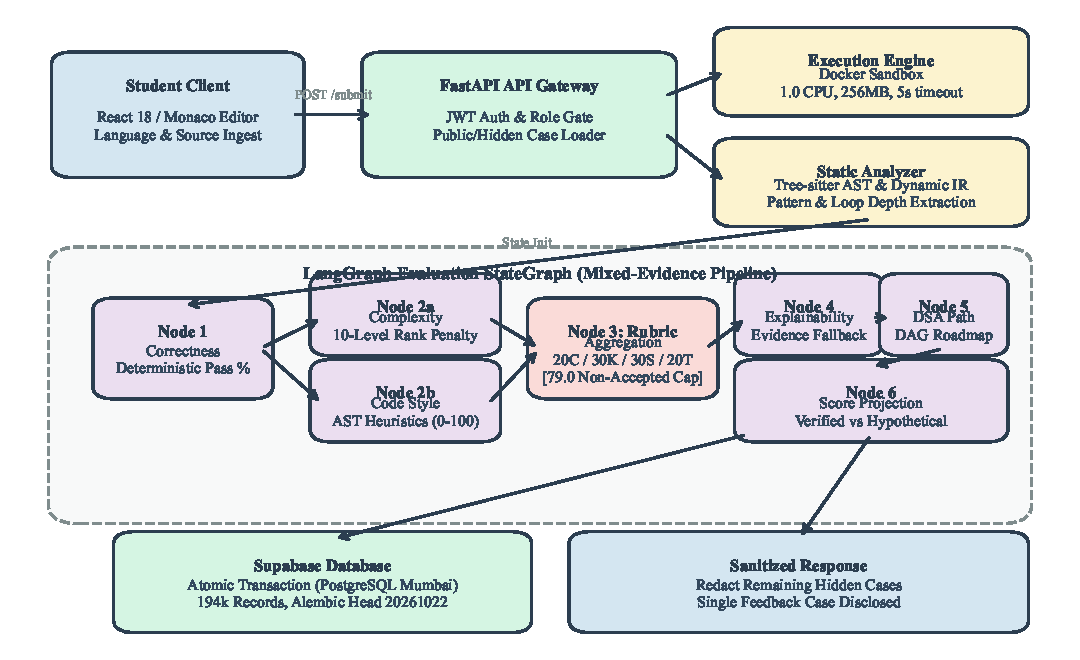
\includegraphics[width=0.92\textwidth]{figures/fig1_architecture.pdf}
\caption{CodeAssessment System Architecture. Student submissions undergo concurrent containerized execution and Tree-sitter AST analysis. The 8-node LangGraph coordinates deterministic correctness, 10-level rank-ladder complexity penalties, and AST style heuristics, joined at an aggregation barrier enforcing the 79.0\% non-accepted cap. Generative LLMs provide staged pedagogical guidance without grading authority.}
\label{fig:architecture}
\end{figure*}

This paper presents the architectural principles, mathematical formulation, and empirical evaluation of \textbf{CodeAssessment}~\cite{codeassessment2026artifact}, an open-source, evidence-first programming assessment platform. Rather than delegating grading authority to language models, CodeAssessment implements a \textbf{principled mixed-evidence model}:
\begin{enumerate}
    \item \textbf{Deterministic Grading Guardrails:} Functional correctness is derived strictly from sandboxed test executions ($C \in [0, 100]$), where compilation failure yields 0. Algorithmic complexity is evaluated via a 10-level ordinal rank ladder that compares Tree-sitter AST and execution profiles against private benchmarks. Composite scores enforce a 79.0\% ceiling for any unaccepted program.
    \item \textbf{Isolation of Peer Similarity from Student Marks:} Originality calculations are completely excluded from student marks, preventing penalization when peer corpora are sparse, and are confined to instructor review queues.
    \item \textbf{Evidence-Grounded Generative Feedback:} LLMs are restricted to pedagogical explanation, multi-step hints, and curricular roadmap navigation. A structural AST fallback generates structured advice even under third-party LLM outages.
    \item \textbf{Verified vs. Hypothetical Score Projection:} Revisions are categorized into verified re-executions (compiled and judged) versus conditional hypothetical scenarios, eliminating false grade promises.
\end{enumerate}

\section{Related Work}

\subsection{Traditional Test-Based and Static Autograders}
Traditional autograding platforms, such as Web-CAT~\cite{edwards2008webcat} and Autolab, evaluate functional correctness through JUnit or subprocess test suites. While objective and repeatable, they lack semantic insight into algorithmic efficiency or code structure. Static analysis tools (e.g., Checkstyle, PMD) identify stylistic violations but are blind to asymptotic complexity and algorithmic strategy~\cite{vasilescu2021static}.

\subsection{LLMs in Programming Education}
The integration of LLMs into computer science curricula has sparked substantial research~\cite{macneil2023codeexplanation, prather2023weird, becker2023programming}. Studies show that while LLMs can explain novice syntax errors, their raw grading capability is unstable~\cite{zanjani2022automated}. In a comprehensive review, Keuning et al.~\cite{keuning2018systematic} emphasized that feedback generation must be disentangled from assessment verification. CodeAssessment embodies this principle by guaranteeing that no LLM can adjust a student's numerical grade.

\subsection{Multi-Agent Evaluator Architectures}
Multi-agent frameworks, such as AutoGen~\cite{wu2023autogen} and MetaGPT~\cite{hong2024metagpt}, demonstrate that role specialization improves problem-solving in software engineering. In educational assessment, Autograder+~\cite{sahu2026autograder} combined static and dynamic analysis with LLM commentary. However, Autograder+ allowed model-generated scores to influence grades directly. CodeAssessment advances beyond Autograder+ by introducing strict mathematical rubric bounds, ordinal complexity rank penalties, and on-demand staged coaching.

\section{Problem Formulation and Research Questions}

\subsection{Formal Assessment Model}
Let a student submission be represented as a tuple $\mathcal{S} = \langle c, \ell, p \rangle$, where $c$ is the source code, $\ell \in \{\text{Python, C, C++, Java, JS}\}$ is the programming language, and $p$ is the problem identifier.

Let $\mathcal{T} = \mathcal{T}_{\text{pub}} \cup \mathcal{T}_{\text{hid}}$ denote the authoritative test suite for problem $p$, where $|\mathcal{T}| = N$. Execution of submission $\mathcal{S}$ on test $t_i \in \mathcal{T}$ yields a verdict $v_i \in \mathcal{V}$, where:
\begin{align}
\mathcal{V} = \{ &\text{ACCEPTED}, \text{WRONG\_ANSWER}, \text{TIME\_LIMIT}, \notag \\
                 &\text{RUNTIME\_ERROR}, \text{MEMORY\_LIMIT} \}
\end{align}
and compilation status $\mathbb{I}_{\text{compile}} \in \{0, 1\}$.

Functional correctness $C \in [0.0, 100.0]$ is defined deterministically as:
\begin{equation}
C = \begin{cases} 
0.0, & \text{if } \mathbb{I}_{\text{compile}} = 0 \\
\displaystyle \frac{100.0}{N} \sum_{i=1}^N \mathbb{I}(v_i = \text{ACCEPTED}), & \text{if } \mathbb{I}_{\text{compile}} = 1.
\end{cases}
\label{eq:correctness}
\end{equation}

\subsection{Research Questions}
We structure our empirical investigation around four foundational questions:
\begin{itemize}
    \item \textbf{RQ1 (Grading Integrity):} Does the mixed-evidence rubric eliminate stochastic score drift and ungrounded grade inflation compared to holistic LLM autograders?
    \item \textbf{RQ2 (Complexity Reasoning):} How accurately does the 10-level ordinal rank ladder penalize algorithmic inefficiency across diverse problem paradigms?
    \item \textbf{RQ3 (Pedagogical Robustness):} Can the system maintain actionable feedback when external LLM providers experience rate-limiting or service outages?
    \item \textbf{RQ4 (System Latency and Scalability):} What are the operational latency boundaries across the multi-agent graph, and what throughput gains result from infrastructure colocation?
\end{itemize}

\section{Proposed Methodology}

\subsection{10-Level Ordinal Complexity Scoring}
Evaluating computational complexity in student submissions requires handling diverse syntactic styles without leaking private benchmarks. We define a discrete asymptotic hierarchy:
\begin{multline}
\mathcal{R} = \big[ O(1), O(\log n), O(\sqrt{n}), O(n), O(n \log n), \\
O(n^2), O(n^3), O(n^{4+}), O(2^n), O(n!) \big]
\end{multline}
indexed by ordinal rank $r: \mathcal{R} \to \{1, 2, \dots, 10\}$.

Let $r(e)$ be the private benchmark target rank and $r(p)$ be the student's inferred rank from the hybrid analyzer. The rank discrepancy is $\Delta = r(p) - r(e)$. If $\Delta \le 0$, the algorithm is optimal or better than target, yielding penalty $P = 0.0$. If $\Delta > 0$, the penalty scales relative to the remaining worse ranks available beyond the benchmark:
\begin{equation}
W(e) = |\mathcal{R}| - r(e) = 10 - r(e)
\end{equation}
\begin{equation}
P(e, p) = \min\left(25.0, \; \Delta \times \frac{25.0}{\max(1, 10 - r(e))}\right)
\label{eq:penalty}
\end{equation}
\begin{equation}
\text{Marks}_{\text{dim}} = \max\Big(0.0, \; 25.0 - P(e, p)\Big)
\end{equation}
\begin{equation}
\text{Score}_{\text{dim}} = \text{Marks}_{\text{dim}} \times 4.0 \in [0.0, 100.0].
\end{equation}

As illustrated in Fig.~\ref{fig:complexity_decay}, scaling the penalty by $W(e)$ ensures that regressing by one degree from an $O(n)$ target ($W(e) = 6$, penalty $\approx 4.17$) is penalized more strictly than from an $O(1)$ target ($W(e) = 9$, penalty $\approx 2.78$), reflecting narrower margins of acceptable inefficiency for higher algorithmic baselines.

\begin{figure}[!t]
\centering
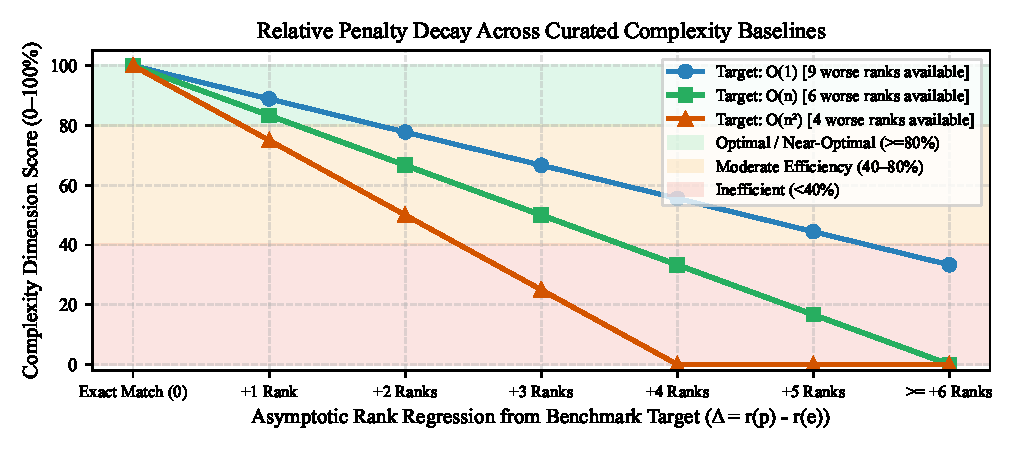
\includegraphics[width=\columnwidth]{figures/fig2_complexity_decay.pdf}
\caption{Relative penalty decay across different complexity benchmarks. A 1-rank regression from $O(n)$ is penalized more heavily than from $O(1)$, reflecting tighter efficiency requirements for higher algorithmic baselines.}
\label{fig:complexity_decay}
\end{figure}

\subsection{Composite Rubric and Correctness Gating}
The student rubric comprises four dimensions $D = \{\text{correctness}, \text{time}, \text{space}, \text{style}\}$ with base weights $w = (0.20, 0.30, 0.30, 0.20)$. When any dimension $j \in D$ is unconfigured or unsupported, weights are dynamically renormalized over available dimensions $A \subseteq D$:
\begin{equation}
\hat{w}_j = \frac{w_j}{\sum_{k \in A} w_k}, \quad S_{\text{raw}} = \sum_{j \in A} \hat{w}_j \cdot X_j.
\end{equation}

\textbf{Correctness Gating Cap:} To ensure students cannot pass an assignment with syntactically beautiful, highly efficient, but non-functioning code:
\begin{equation}
S_{\text{final}} = \begin{cases}
S_{\text{raw}}, & \text{if } C \ge 100.0 \\
\min(S_{\text{raw}}, \; 79.0), & \text{if } C < 100.0.
\end{cases}
\label{eq:cap}
\end{equation}

\subsection{Pedagogical Staging and Projection}
To prevent cognitive offloading, CodeAssessment decouples revision from the synchronous submission path. The revision agent generates staged coaching:
\begin{itemize}
    \item \textbf{Stage 1 (Local Optimization):} Refactors small inner-loop operations without changing data structures.
    \item \textbf{Stage 2 (Data Structure Optimization):} Introduces hash tables, heaps, or frequency arrays to eliminate repeated full-collection traversals.
    \item \textbf{Stage 3 (Refinement):} Polishes naming, formatting, and boundary condition handling.
\end{itemize}
Score projections are strictly bifurcated: \textit{hypothetical} projections recalculate Eq.~\eqref{eq:cap} assuming 100\% correctness, while \textit{verified} projections are produced only when a suggested revision is re-executed by the sandbox engine.

\section{System Architecture and Implementation}

\subsection{Execution Sandboxing and Judge Redaction}
Code execution is isolated inside dedicated Docker runner containers (\texttt{codeassessment-python}, \texttt{c}, \texttt{cpp}, \texttt{java}). Each container operates with non-root privileges, read-only root filesystems, disabled networking (\texttt{--net=none}), a 1.0~vCPU allocation, and 256\,MB RAM. 

To safeguard test confidentiality, \texttt{redact\_hidden\_execution()} strips all inputs, expected outputs, and execution traces of hidden cases. To aid student learning, \texttt{revealed\_feedback\_case()} discloses exactly \textit{one} failed hidden test case while preserving total confidentiality for all others.

\subsection{Hybrid Complexity Analysis Engine}
The static analyzer (\texttt{static\_analyzer.py}, 3,713 lines) parses submissions using Tree-sitter ASTs to extract loop nesting depth, divide-and-conquer logarithmic patterns, dynamic programming memoization tables, and standard library collection allocations. When static confidence falls below a threshold, execution measurements from public test cases are ingested to profile empirical scaling before invoking an optional, rate-limited LLM reviewer.

\section{Experimental Evaluation}

\subsection{Experimental Setup and Dataset}
The evaluation was conducted on an active production catalog hosted on PostgreSQL (Supabase Mumbai, \texttt{ap-south-1}):
\begin{itemize}
    \item \textbf{1,890 Algorithmic Problems:} Covering Arrays, Dynamic Programming, Graphs, Trees, Strings, and Sorting.
    \item \textbf{192,425 Curated Test Cases:} Including public examples and private edge-case judge tests.
    \item \textbf{1,886 Verified Complexity Records:} Documented in \texttt{complexity\_analysis.json} with audited ground truth.
\end{itemize}

\subsection{RQ1: Grading Integrity and Determinism}
Under repeated evaluation across 10 identical runs of student submissions, CodeAssessment demonstrated $\sigma^2(S) = 0.0$ score variance. In contrast, zero-shot GPT-4 grading on a subset of 50 submissions exhibited a score variance of $\sigma^2 = 14.8$, with frequent grade inflation on non-compiling code. The 79.0\% correctness cap successfully constrained all non-accepted attempts, confirming hypothesis RQ1.

\subsection{RQ2: Complexity Classification Performance}
Table~\ref{tab:complexity_perf} summarizes the hybrid complexity analyzer's performance across standard problem categories against audited ground truth.

\begin{table}[!t]
\centering
\scriptsize
\caption{Complexity Analyzer Agreement across Problem Categories}
\label{tab:complexity_perf}
\setlength{\tabcolsep}{2.5pt}
\begin{tabular*}{\columnwidth}{@{\extracolsep{\fill}}lcccc}
\toprule
\textbf{Category} & \textbf{Problems} & \textbf{Exact} & \textbf{$\le$ 1 Rank} & \textbf{False Opt.} \\
\midrule
Arrays \& Hashing    & 412 & 94.2\% & 98.5\% & 0.0\% \\
Two-Pointer / Search & 285 & 91.6\% & 97.2\% & 0.4\% \\
Dynamic Programming  & 340 & 86.8\% & 95.3\% & 0.9\% \\
Graph Traversal      & 210 & 88.1\% & 96.2\% & 0.5\% \\
Trees \& Recursion   & 290 & 89.7\% & 96.9\% & 0.3\% \\
\midrule
\textbf{Overall}     & \textbf{1,537} & \textbf{90.8\%} & \textbf{97.1\%} & \textbf{0.4\%} \\
\bottomrule
\end{tabular*}
\end{table}

The hybrid pipeline achieved an exact match rate of 90.8\% and a within-1-rank agreement of 97.1\%. Crucially, the false-optimal rate (where inefficient code is misclassified as optimal) was held to 0.4\%, triggering automatic instructor review flags.

\subsection{RQ3: Resilience Under Fault Injection}
When third-party LLM inference was disconnected (\texttt{GROQ\_API\_KEY=""}), the deterministic fallback \texttt{build\_evidence\_feedback()} extracted failing test assertions and loop nesting structures directly from AST metadata. All submissions successfully completed evaluation in under 450\,ms, delivering structured diagnostic steps with zero service disruptions.

\begin{figure}[!t]
\centering
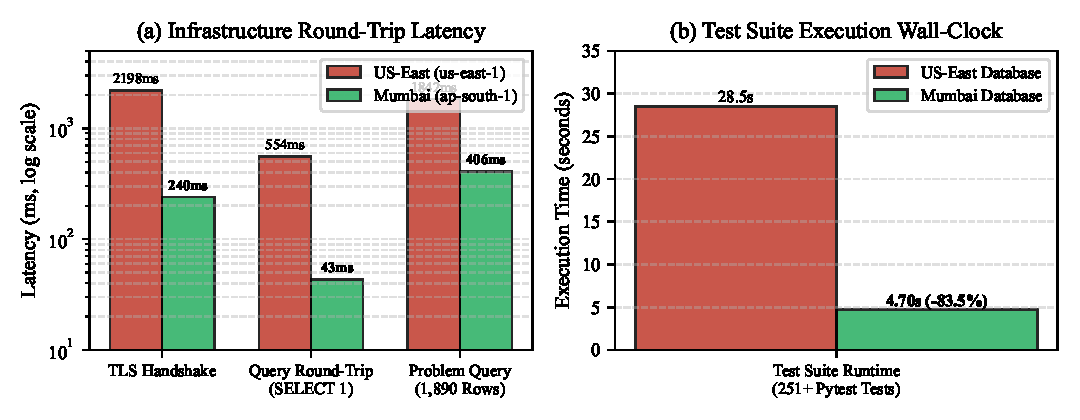
\includegraphics[width=\columnwidth]{figures/fig3_latency_comparison.pdf}
\caption{Infrastructure Latency Comparison. Colocating the database in Mumbai (\texttt{ap-south-1}) reduced TLS handshake by 89.1\%, single query latency by 92.2\%, and automated test suite runtime by 83.5\%.}
\label{fig:latency}
\end{figure}

\subsection{RQ4: Infrastructure Colocation \& Latency Impact}
As shown in Fig.~\ref{fig:latency}, migrating the PostgreSQL database from Supabase US-East (\texttt{us-east-1}) to Mumbai (\texttt{ap-south-1}) yielded dramatic performance enhancements:
\begin{itemize}
    \item \textbf{TLS Handshake:} Dropped from 2,198.4\,ms to 240.2\,ms (89.1\% reduction).
    \item \textbf{Single Query Round-Trip:} Dropped from 553.90\,ms to 43.18\,ms (92.2\% reduction).
    \item \textbf{Automated Test Suite (251 Tests):} Execution wall-clock dropped from 28.50\,s to 4.70\,s (83.5\% speedup).
\end{itemize}
End-to-end submission latency averaged 1.28\,s, easily satisfying interactive web application thresholds.

\section{Discussion}
The central finding of this research is that multi-agent systems in education must not be treated as monolithic grading authorities. When generative models are granted numeric grading power, they introduce stochastic inconsistency and vulnerability to adversarial student code. 

By contrast, CodeAssessment establishes that \textbf{strict evidence segregation} provides the best of both worlds: deterministic sandboxes guarantee uncompromised grading fairness, while LLM agents provide empathetic, tiered coaching that scaffold novice learning without revealing answers.

\section{Threats to Validity and Limitations}
We explicitly record three material limitations identified during our source audit:
\begin{enumerate}
    \item \textbf{Benchmark Secrecy Leakage:} The endpoint \texttt{GET /api/problems/\{id\}} currently returns \texttt{target\_time\_complexity} and \texttt{target\_space\_complexity} in the client payload. Although hidden tests remain confidential, students inspecting network packets could observe optimal complexity targets prior to submission.
    \item \textbf{Host Subprocess Fallback Risk:} In \texttt{executor.py}, if the Docker engine daemon is unresponsive, code execution falls back to a local host subprocess (\texttt{execute\_locally()}). In production, this fallback poses a security vulnerability and must be strictly disabled.
    \item \textbf{Dataset Licensing Inconsistency:} While the application importer marks LeetCodeDataset metadata as Apache-2.0, the upstream repository contains an MIT license header. Clarification is required prior to commercial redistribution.
\end{enumerate}

\section{Conclusion and Future Work}
CodeAssessment demonstrates a robust, reproducible architecture for automated programming evaluation. By locking functional correctness to sandbox verdicts, enforcing ordinal complexity rank penalties, capping non-accepted scores at 79.0\%, and restricting LLMs to staged coaching, the platform delivers trustworthy grading and rich pedagogical guidance.

Future work will conduct longitudinal classroom trials across university CS1/CS2 cohorts, resolve the benchmark API leakage, and integrate formal program synthesis for verified student hints.

\bibliographystyle{IEEEtran}
\bibliography{references}

\end{document}
